% Tikz File 'fig_07_stateDiagram.tex'
\documentclass{standalone}
\usepackage{tikz}
\usetikzlibrary{positioning}
\begin{document}
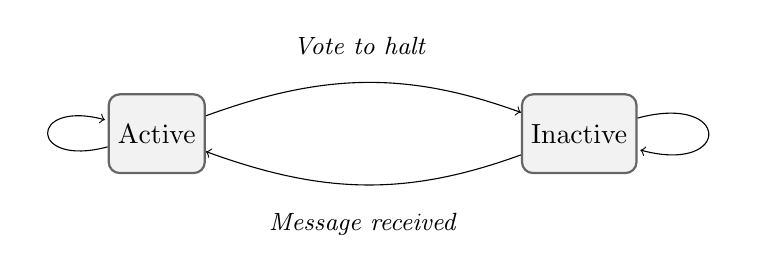
\begin{tikzpicture}[
        activenode/.style={rectangle, rounded corners, draw=black!60, fill=black!5, thick, minimum size=10mm},
    ]
    \node[activenode] (active)                     {Active};
    \node[activenode] (inactive) [right=4cm of active] {Inactive};

    \path[-to,in=180-20,out=0+20] (active) edge node[above=2.36mm,pos=.49] {\small \textit{Vote to halt}} (inactive);
    \path[to-,in=180+20,out=0-20] (active) edge node[below=2.36mm] {\small \textit{Message received}} (inactive);
    \path[-to] (active)   edge[loop left]  node {} (active);
    \path[-to] (inactive) edge[loop right] node {} (inactive);
\end{tikzpicture}
\end{document}